
\documentclass[conference]{IEEEtran}\usepackage[]{graphicx}\usepackage[]{color}
%% maxwidth is the original width if it is less than linewidth
%% otherwise use linewidth (to make sure the graphics do not exceed the margin)
\makeatletter
\def\maxwidth{ %
  \ifdim\Gin@nat@width>\linewidth
    \linewidth
  \else
    \Gin@nat@width
  \fi
}
\makeatother

\definecolor{fgcolor}{rgb}{0.345, 0.345, 0.345}
\newcommand{\hlnum}[1]{\textcolor[rgb]{0.686,0.059,0.569}{#1}}%
\newcommand{\hlstr}[1]{\textcolor[rgb]{0.192,0.494,0.8}{#1}}%
\newcommand{\hlcom}[1]{\textcolor[rgb]{0.678,0.584,0.686}{\textit{#1}}}%
\newcommand{\hlopt}[1]{\textcolor[rgb]{0,0,0}{#1}}%
\newcommand{\hlstd}[1]{\textcolor[rgb]{0.345,0.345,0.345}{#1}}%
\newcommand{\hlkwa}[1]{\textcolor[rgb]{0.161,0.373,0.58}{\textbf{#1}}}%
\newcommand{\hlkwb}[1]{\textcolor[rgb]{0.69,0.353,0.396}{#1}}%
\newcommand{\hlkwc}[1]{\textcolor[rgb]{0.333,0.667,0.333}{#1}}%
\newcommand{\hlkwd}[1]{\textcolor[rgb]{0.737,0.353,0.396}{\textbf{#1}}}%

\usepackage{framed}
\makeatletter
\newenvironment{kframe}{%
 \def\at@end@of@kframe{}%
 \ifinner\ifhmode%
  \def\at@end@of@kframe{\end{minipage}}%
  \begin{minipage}{\columnwidth}%
 \fi\fi%
 \def\FrameCommand##1{\hskip\@totalleftmargin \hskip-\fboxsep
 \colorbox{shadecolor}{##1}\hskip-\fboxsep
     % There is no \\@totalrightmargin, so:
     \hskip-\linewidth \hskip-\@totalleftmargin \hskip\columnwidth}%
 \MakeFramed {\advance\hsize-\width
   \@totalleftmargin\z@ \linewidth\hsize
   \@setminipage}}%
 {\par\unskip\endMakeFramed%
 \at@end@of@kframe}
\makeatother

\definecolor{shadecolor}{rgb}{.97, .97, .97}
\definecolor{messagecolor}{rgb}{0, 0, 0}
\definecolor{warningcolor}{rgb}{1, 0, 1}
\definecolor{errorcolor}{rgb}{1, 0, 0}
\newenvironment{knitrout}{}{} % an empty environment to be redefined in TeX

\usepackage{alltt}

\date{\today}
\usepackage[cmex10]{amsmath}
\usepackage{algorithmicx}
\usepackage{algpseudocode}

\usepackage[english]{babel}


\usepackage{url}




% *** GRAPHICS RELATED PACKAGES ***
% 
\ifCLASSINFOpdf
% \usepackage[pdftex]{graphicx}
% declare the path(s) where your graphic files are
% \graphicspath{{../pdf/}{../jpeg/}}
% and their extensions so you won't have to specify these with
% every instance of \includegraphics
% \DeclareGraphicsExtensions{.pdf,.jpeg,.png}
\else
% or other class option (dvipsone, dvipdf, if not using dvips). graphicx
% will default to the driver specified in the system graphics.cfg if no
% driver is specified.
% \usepackage[dvips]{graphicx}
% declare the path(s) where your graphic files are
% \graphicspath{{../eps/}}
% and their extensions so you won't have to specify these with
% every instance of \includegraphics
% \DeclareGraphicsExtensions{.eps}
\fi
% graphicx was written by David Carlisle and Sebastian Rahtz. It is
% required if you want graphics, photos, etc. graphicx.sty is already
% installed on most LaTeX systems. The latest version and documentation
% can be obtained at: 
% http://www.ctan.org/tex-archive/macros/latex/required/graphics/
% Another good source of documentation is "Using Imported Graphics in
% LaTeX2e" by Keith Reckdahl which can be found at:
% http://www.ctan.org/tex-archive/info/epslatex/
% 
% latex, and pdflatex in dvi mode, support graphics in encapsulated
% postscript (.eps) format. pdflatex in pdf mode supports graphics
% in .pdf, .jpeg, .png and .mps (metapost) formats. Users should ensure
% that all non-photo figures use a vector format (.eps, .pdf, .mps) and
% not a bitmapped formats (.jpeg, .png). IEEE frowns on bitmapped formats
% which can result in "jaggedy"/blurry rendering of lines and letters as
% well as large increases in file sizes.
% 
% You can find documentation about the pdfTeX application at:
% http://www.tug.org/applications/pdftex





% correct bad hyphenation here
\hyphenation{op-tical net-works semi-conduc-tor}
\IfFileExists{upquote.sty}{\usepackage{upquote}}{}
\begin{document}
% 
% paper title
% Titles are generally capitalized except for words such as a, an, and, as,
% at, but, by, for, in, nor, of, on, or, the, to and up, which are usually
% not capitalized unless they are the first or last word of the title.
% Linebreaks \\ can be used within to get better formatting as desired.
% Do not put math or special symbols in the title.
\title{Predicting the Number of Shares of a Webpage}


% author names and affiliations
% use a multiple column layout for up to three different
% affiliations
\author{\IEEEauthorblockN{Alexandre Piche}
  \IEEEauthorblockA{ 260478404 \\
  }
  \and
  \IEEEauthorblockN{Philippe Nguyen}
  \IEEEauthorblockA{260482336 \\
  }
  \and
  \IEEEauthorblockN{Yash Lakhani}
  \IEEEauthorblockA{260500612\\
  }}



% make the title area
\maketitle



% As a general rule, do not put math, special symbols or citations
% in the abstract
\begin{abstract}
  We implementated a linear regression using the Ordinary Least Square and the
  Maximum Likelihood methods. Trying to improve our prediction power, we also
  explored dimension reduction, and regularization methods
\end{abstract}

% no keywords




\IEEEpeerreviewmaketitle


\section{Introduction}

In the advertising industry, it is of interest to predict the popularity of an
article to adequately set the price of the ads that will appear on its page.


\section{Datasets}

We first used a publicly available dataset available on the UCI Machine Learning
repository. We also created our own dataset using articles from the Huffington Post.

\subsection{Mashable Dataset} 

39,000 Mashable articles were collected from January 7 2013 to January 7 2015 by
???. Note that article with less of 3 weeks of existence were discarded since
it is probable that the number of share have not converge.

It contains features such as word count, number of links

A comprehensive overview of the data is available on UCI Machine Learning
repository \cite{Lichman:2013}. 

Achieve the best results on this dataset by using Random Forest.
\cite{fernandes2015proactive}  

\subsection{Huffington Post Dataset}

\section{Implementation of Linear Regression}

Ordinary least square is a simple and surprisingly powerful tool for prediction.
$Y$ is the target value, $X$ is the covariates and $\beta$ is the weights of
those covariates.

\begin{eqnarray*}
  Y = X \beta + \epsilon
\end{eqnarray*}


\subsection{Least Squares Estimate}

With the traditional assumption of $E(X^T \epsilon) = 0$
\cite{davidson2004econometric}, i.e. that the error is 
uncorrelated with the matrix $X$, it is easy to solve for the weights, the
resulting equation is given by

\begin{eqnarray*}
  Y &=& X \beta + \epsilon \\
  X^T Y &=& X^T X \beta + X^T \epsilon \\
  \hat{\beta} &=& (X^TX)^{-1}X^TY 
\end{eqnarray*}

It is possible to weaken the assumption that $E(X^T \epsilon) = 0$, namely to
deal with heteroskedasticity. The method is called 
\textit{Generalized Least Squared} and is well explained in
\cite{davidson2004econometric}. However due to it's computational complexity 
this method was not carried in this experiment.   

\subsection{Maximum Likelihood Estimate}

Assuming that the error $\epsilon \sim \mathcal{N}(0, \sigma^2)$ it is possible
to show that the maximum likelihood method yields the same solution than the
closed solution.

\begin{eqnarray*}
  f_t(y_t, \beta, \sigma) &=& \frac{1}{\sigma \sqrt{2 \pi}} \exp \Bigg(-
                              \frac{(y_t-X_t \beta)^2}{2 \sigma^2} \Bigg)
\end{eqnarray*}

It can be easily show that by taking the log of the likelihood and summing over
$n$, since the observations are assumed to be independent, gives the following
log-likelihood: 

\begin{eqnarray*}
  l(y, \beta, \sigma) &=& -\frac{n}{2} \log 2 \pi - \frac{n}{2} \log \sigma^2
                            - \frac{1}{2 \sigma^2} (y - X \beta)^2
\end{eqnarray*}

Differentiating the log likelihood with respect to $\sigma$ yields

\begin{eqnarray*}
  \frac{\partial l(y, \beta, \sigma)}{\partial \sigma} &=& - \frac{n}{\sigma} +
                                                           \frac{1}{\sigma^3}
                                                           (y-X\beta)^T(y - X \beta)
\end{eqnarray*}

Setting the derivative equal to zero yields

\begin{eqnarray*}
  \sigma^2(\beta) &=& \frac{1}{n}(y-X \beta)^T(y-X \beta)
\end{eqnarray*}

which minimizes the variance. Substituting in the likelihood function yields

\begin{eqnarray*}
  l(y, \beta) &=& -\frac{n}{2} \log 2 \pi - \frac{n}{2} \log
                  \Big(\frac{1}{n}(y-X \beta)^T (y-X \beta) \Big) - \frac{n}{2}
\end{eqnarray*}

Since only the second term contains $\beta$ and by the properties of the $\log$
the problem then boils up to minimize the $SSR(\beta) = (y-X \beta)^T (y-X
\beta)$. We can take the derivative with respect to $\beta$ (gradient).

\begin{eqnarray*}
  \frac{\partial SSR(\beta)}{\partial \beta} &=& -2 X^T (Y-X \beta)
\end{eqnarray*}

A coverage in depth of this derivation can be found in
\cite{davidson2004econometric}

To maximize the likelihood (minimize the SSR) we need to implement a gradient
descent algorithm. 

\begin{algorithmic}
  \While {$\epsilon > 0.1$ and $i < \text{max\_iterations}$}
  \State hypothesis $\leftarrow$ $X^T \beta$
  \State loss $\leftarrow$ hypothesis - $Y$
  \State gradient $\leftarrow$ 2 $X^T$ loss
  \State $\beta_{\text{new}} \leftarrow \beta - \frac{\alpha *
    \text{gradient}}{n}$  
  \State $\epsilon \leftarrow \| \beta_{\text{new}} - \beta \| $ 
  \State $i \leftarrow i + 1$
  \State $\beta_{\text{new}} \leftarrow \beta$
  \EndWhile
\end{algorithmic}

\subsection{Model selection}

It is sometimes useful to take into consideration the variance of our
coefficients to determine whether or not they should be part of our model.
Traditional statistics came up with multiple tools to assess the predictive
power of a model based on the likelihood and the variance of the coefficients.
We will cover some of the more useful in this section.

Only having the size of the weights is of little used if we cannot asses the fit
of the model.

\subsubsection{Significance of our Weights}

It is possible that even if the weight is big that the variance is so high that
it is not significantly different from zero.

\begin{eqnarray*}
  Var(\hat{\beta}) &=& s^2 (X^TX)^{-1} \\
  s^2 &=& \frac{1}{n-k} \sum_{t=1}^n \hat{u}_t^2
 \end{eqnarray*}
\cite{davidson2004econometric}
\subsubsection{Adjusted $R^2$}

To asses the fit of the model, it is helpful to look at the percentage of the
sum of square that is explained by our model.

\begin{eqnarray*}
  \bar{R}^2 &=& 1 - \frac{\frac{1}{n-k}\sum_{t=1}^n
                \hat{u}_t^2}{\frac{1}{n-1}\sum_{t=1}^n (y_t-\bar{y})^2}
\end{eqnarray*}
\cite{davidson2004econometric}
\subsubsection{AIC and BIC}

It is possible to select a model based on the information criteria. It is
particularly useful to test the difference between two nonnested models.


Adding a variable cannot decrease the fit and almost always increase the
prediction power of the model. However it might add noise to the prediction. AIC
and BIC are a way to quantify the importance of adding a feature to our model by
penalizing complexity.

Akaike information criterion is given by

\begin{eqnarray*}
  \text{AIC}_i &=& l_i(\hat{\theta}_i) - k_i
\end{eqnarray*}

Bayesian information criterion

\begin{eqnarray*}
  \text{BIC}_i &=& l_i(\hat{\theta}_i) - \frac{1}{2} k_i \log n
\end{eqnarray*}


\cite{davidson2004econometric}

\section{Model Complexity and Dimension Reduction}

There is a total of 59 features, where some of them are correlated. Given the
high number of features, it might be preferable to reduce the dimension to
achieve better out of sample prediction. The intuition is that too many
features will increase the variance of our weight estimates while too few
features will lead our model to be bias.

It is also along the reasoning line of the widely accepted Occam's razor
principle. The principle suggests that parsimonous models generalize better than
more complex model.  

There is multiple way to avoid an over complex model that will generalize well
for prediction, we will explore the performance of some of the most known of
them. 

\subsection{Principal Component Analysis}

Given the large dimension of the dataset and that some of the feature are highly
correlated we decided to the principal component analysis algorithm to reduce
the dimension by using  
principal component analysis (PCA) algorithm. We noticed that over $95\%$ of the
variance can be explained by the first $22$ dimensions. The idea behind the PCA
algorithm is trying to reconstruct X, by the minimal set of component. Namely we
want to find a $W$ such that 

$L$ linear basis vector

$X$ is $K \times N$, where $K$ is the number of feature and $N$ the number of
examples. 

\begin{eqnarray*}
  J(W, Z) &=& \| X - WZ^T\|_F^2
\end{eqnarray*}

Frobenius norm.

Where $W$ is $K \times L$ orthonormal and $Z$ is $N \times L$ matrix

\cite{murphy2012machine}
\cite{scikit-learn}

\subsection{Ridge or L2-Regularization}

\begin{eqnarray*}
  \hat{\beta}^{\text{ridge}} = \stackrel{\text{argmin}}{\beta}
  \Bigg\{ \sum_{i=1}^N \bigg(y_i - \beta_0 \sum_{j=1}^p x_{ij} \beta_j \bigg)^2 +
  \lambda \sum_{j=1}^p \beta_j^2 \Bigg\}
\end{eqnarray*}
\cite{hastie2005elements}

The gradient will then be 

\begin{eqnarray*}
  \frac{\partial SSR(\hat{\beta}^{\text{ridge}} )}{\partial
  \hat{\beta}^{\text{ridge}}} = -2 X^T (Y-X \beta) + 2 \lambda \| \beta \|
\end{eqnarray*}

We can then add the following condition to our gradient descent algorithm

\begin{algorithmic}
  \If {'Ridge' is True}
  \State loss $+= 2 * \lambda \| \beta \|$
  \EndIf
\end{algorithmic}


Ridge regression can also be incorporated fairly easily to OLS 

\begin{eqnarray*}
 \hat{\beta} = (X^TX + \lambda I)^{-1}X^TY
\end{eqnarray*}

Here, $\lambda$ is a hyper-parameter that we can change and optimize using cross validation. A larger $\lambda$ gives a greater amount of regularization. Having $\lambda = 0$ means no L2 regularization, giving the standard ordinary least squares solution.

\subsection{Lasso or L1-Regularization}

Lasso can be used for features selection by setting some of the coefficients to
zero. Note that we should be careful in dropping features because it might
increase the bias of our model, however it will reduce it's variance.

\begin{eqnarray*}
  \hat{\beta}^{\text{lasso}} = \stackrel{\text{argmin}}{\beta}
  \Bigg\{ \sum_{i=1}^N \bigg(y_i - \beta_0 \sum_{j=1}^p x_{ij} \beta_j \bigg)^2 +
  \lambda \sum_{j=1}^p | \beta_j | \Bigg\}
\end{eqnarray*}

There's no closed form solution for the lasso, since the solution is non-linear
(due to the absolute value) \cite{hastie2005elements}. We used the python
library "Scikit Learn" \cite{scikit-learn} to estimate the lasso parameters.

\subsection{Feature Normalization}

It is numerically challenging to apply the gradient to feature that are of
multiple order different from each other. We can normalize without changing
the span of the columns (features), by applying a linear transformation to it.

\section{Cross-Validation}

To optimize the value of our hyperparameters, we train our model on $k-1$ fold
using a particular choice of hyperparameter and then compute a metric of their
predictive performance on the $k$-th fold. We repeated the procedure $k$ times
such as every fold has been used for prediction. We then average the error
across the $k$ experiments and compare the performance.

Formally, our cross validation is done by choosing a $k$, which is the number of
cross 
validation folds. We split the entire data set into $k$ different splits, such
that each split has the same number of instances. If the data set is not divided
equally by $k$, the remainder is added to the last split. We shall use $X[i]$ and
$Y[i]$ to denote split $i$ of the data set. 
\begin{algorithmic}
\State Shuffle the pair $\{X, Y\}$
\For{ fold $i$ }
    \State Set $X[i]$ to be the validation feature matrix
    \State Set $Y[i]$ to be the validation response vector
    \State Combine all other $X[-i]$ to be the training feature matrix
    \State Combine all other $X[-i]$ to be the training response vector
    
    \For {every hyper-parameter setting}
        \State Train the linear model with the current training set and given hyper-parameters
        \State Generate a prediction for $Y$ given the validation feature matrix $X[i]$
        \State Record the error between the predicted $\hat{Y}$ and $Y[i]$
    \EndFor
    
\EndFor
\State Average the error for each hyper-parameter setting across every fold
\State Choose the hyper-parameter setting with the lowest average error
\end{algorithmic}

\section{Results}

Also talk about the $\alpha$ parameter for the gradient descent.

Talk about the mean squared error (MSE) obtain when we varied the alpha of the lasso 
\begin{knitrout}
\definecolor{shadecolor}{rgb}{0.969, 0.969, 0.969}\color{fgcolor}
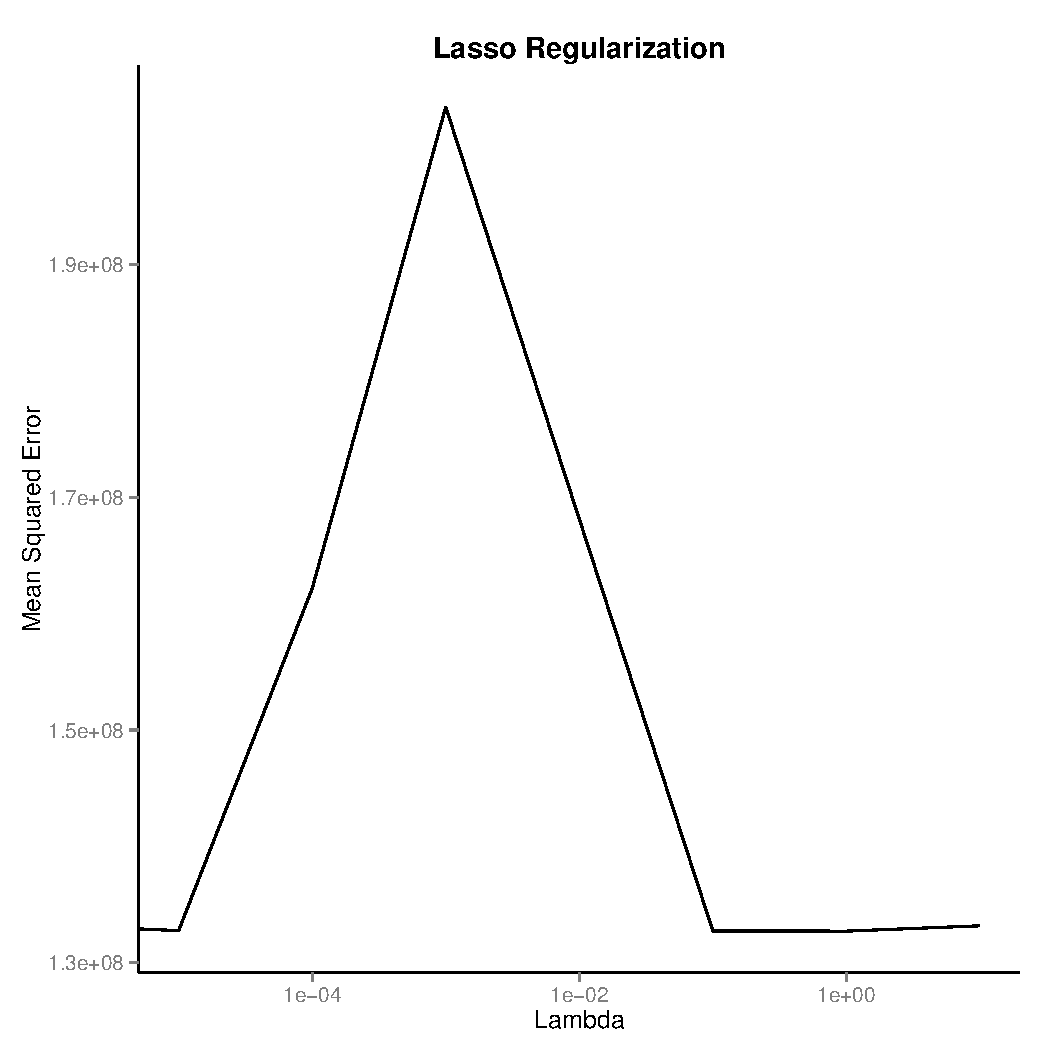
\includegraphics[width=\maxwidth]{figure/unnamed-chunk-2-1} 

\end{knitrout}

\begin{knitrout}
\definecolor{shadecolor}{rgb}{0.969, 0.969, 0.969}\color{fgcolor}
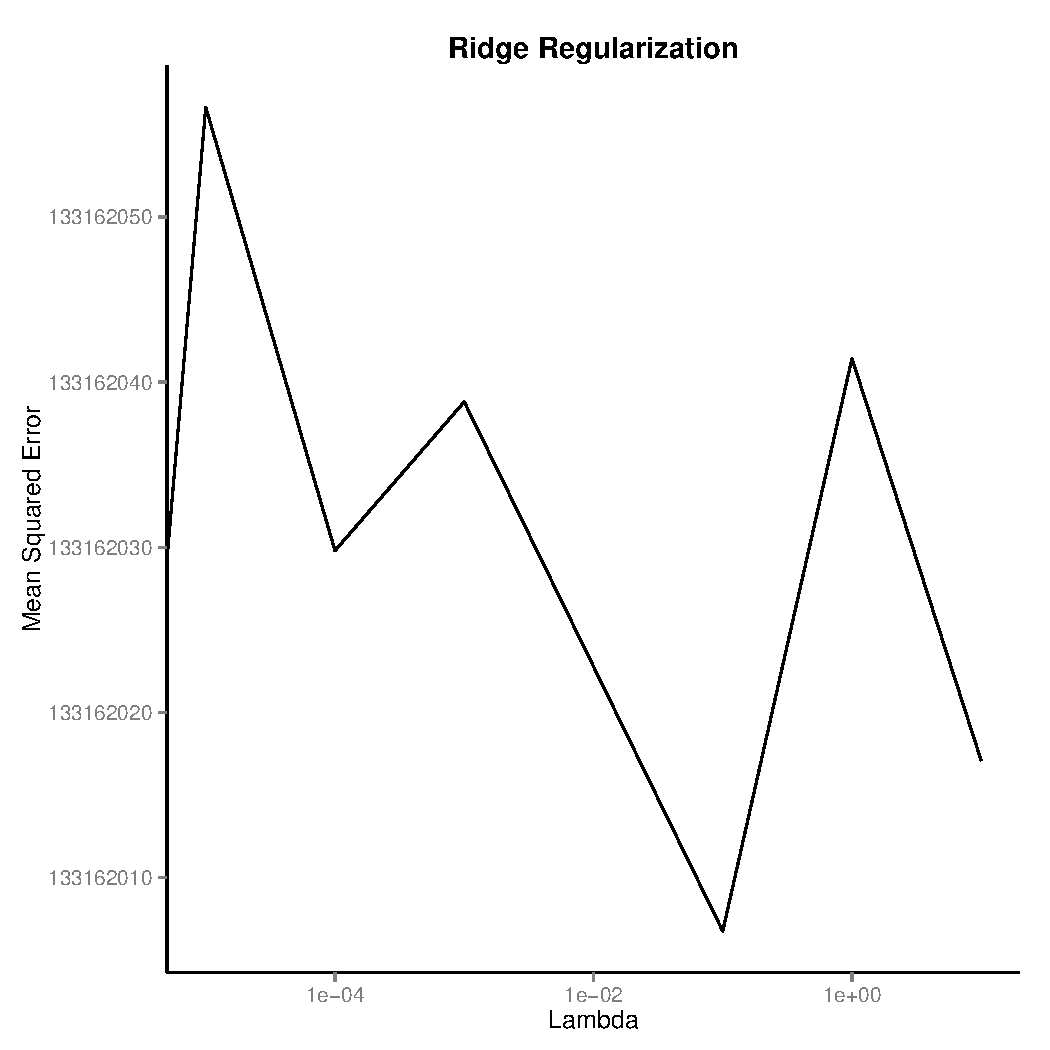
\includegraphics[width=\maxwidth]{figure/unnamed-chunk-3-1} 

\end{knitrout}


\begin{center}
    \begin{tabular}{| l | l |}
    \hline
    \textbf{Algorithm} & \textbf{Mean Squared Error}  \\ \hline
    OLS & 132736810 \\ \hline
    Lasso & \textbf{132712496}  \\ \hline
    Ridge & 133162007  \\ \hline
    Principal component analysis & 133592746  \\ \hline
    \end{tabular}
\end{center}

Lasso is the method that give us the best performance. 

It is probably due to the fact that it is shrinking the coefficients of some
features to zero which was bringing noise to the model instead of increasing
it's predictive power.

Since it is the only
method that we did not implemented, this might be explained by the fact that the
scikit learn library use a better optimization algorithm than the simple
gradient descent than we used.


Given the small difference it might be worth to take the difference in results
with a pinch of salt, since it might not be significant.

\section{Conclusion}

Given our large error linear regression might not be an appropriate tool to
model the popularity of an article. It is possible that the features are not
related in any linear fashion to the number of shares that an article will get.




% trigger a \newpage just before the given reference
% number - used to balance the columns on the last page
% adjust value as needed - may need to be readjusted if
% the document is modified later
% \IEEEtriggeratref{8}
% The "triggered" command can be changed if desired:
% \IEEEtriggercmd{\enlargethispage{-5in}}

% references section

% can use a bibliography generated by BibTeX as a .bbl file
% BibTeX documentation can be easily obtained at:
% http://www.ctan.org/tex-archive/biblio/bibtex/contrib/doc/
% The IEEEtran BibTeX style support page is at:
% http://www.michaelshell.org/tex/ieeetran/bibtex/
% argument is your BibTeX string definitions and bibliography database(s)
% \bibliography{IEEEabrv,../bib/paper}
% 
% <OR> manually copy in the resultant .bbl file
% set second argument of \begin to the number of references
%   (used to reserve space for the reference number labels box)


%   can use a bibliography generated by BibTeX as a .bbl file
%   BibTeX documentation can be easily obtained at:
%   http://www.ctan.org/tex-archive/biblio/bibtex/contrib/doc/
%   The IEEEtran BibTeX style support page is at:
%   http://www.michaelshell.org/tex/ieeetran/bibtex/
\bibliographystyle{IEEEtran}
% argument is your BibTeX string definitions and bibliography database(s)
\bibliography{Bibliography}
% 
% <OR> manually copy in the resultant .bbl file
% set second argument of \begin to the number of references
%   (used to reserve space for the reference number labels box)



%   that's all folks
\end{document}


